\documentclass[a4paper,11pt]{article}
\usepackage[latin1]{inputenc}
\usepackage[T1]{fontenc}
\usepackage{bbm}
\usepackage{amsmath}
\usepackage{indentfirst}
\usepackage{fullpage}
\usepackage{url}
\usepackage{graphicx}
\usepackage[center,footnotesize]{caption}
\usepackage[section]{placeins}
\usepackage{subfig}
\title{Series 5 - BLAST exercise solutions}
\date{October 18, 2011}
\author{Genomics and bioinformatics - Week 5}
\begin{document}
\maketitle

WORK IN PROGRESS..... 

\section{BLAST}

\begin{enumerate}
\item Do you get any matches to \texttt{fragment\_007}? Which parameters did you use? Record the alignment statistics for the top hits.

Using the Nucleotide Collection (nr/nt) Database and optimizing for "more dissimilar sequences"
(discontiguous megablast)

\vspace{0.5cm}
\begin{center}
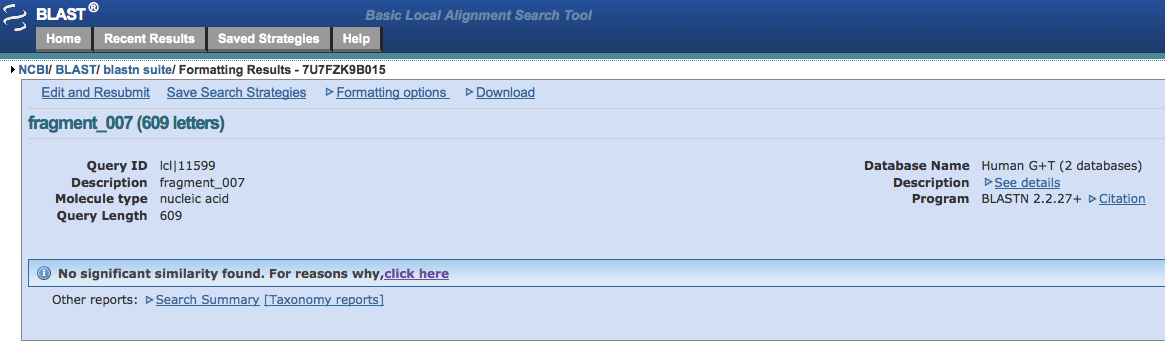
\includegraphics[width=0.8\textwidth]{blastn1.png}
\end{center}
\vspace{0.5cm}

\item Extract the sequence of the hit with the highest query coverage (this may not necessarily be the top hit) and perform another nucleotide BLAST, using the same parameters. Record the alignment statistics for the top hits.

\vspace{0.5cm}
\begin{center}
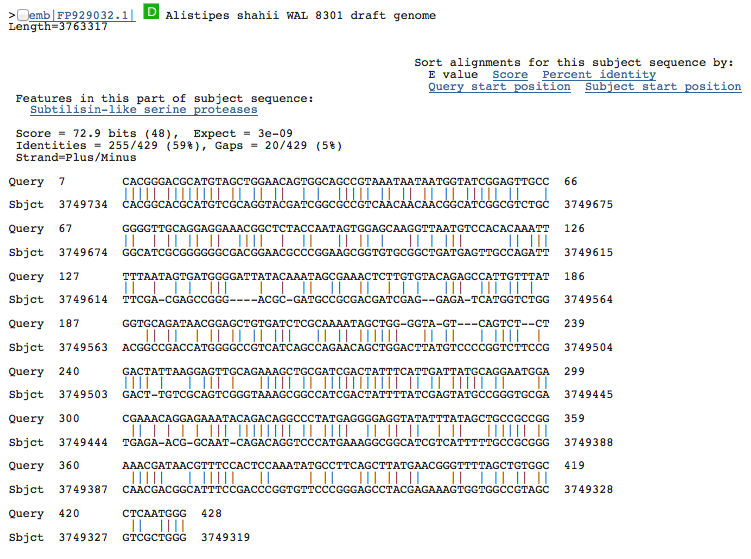
\includegraphics[width=0.8\textwidth]{blastn2.png}
\end{center}
\vspace{0.5cm}

\item What changes do you observe in the E-values? To which parameter could you attribute the these changes?  

Improvement in the E-values. Parameter - Query coverage.

\item What is the default threshold for the E-value on NCBI BLAST?

10

\item Do you have any significant hits suggesting a possible function for \texttt{fragment\_007}? 

The E-values are not significant. 

\end{enumerate}

\subsection{Protein BLAST}

\begin{enumerate}
\item Are any well-known protein domains found? 

Peptidases S8 S53 superfamily

\item Do you get any significant hits? Record the alignment statistics for the top hits. 

\vspace{0.5cm}
\begin{center}
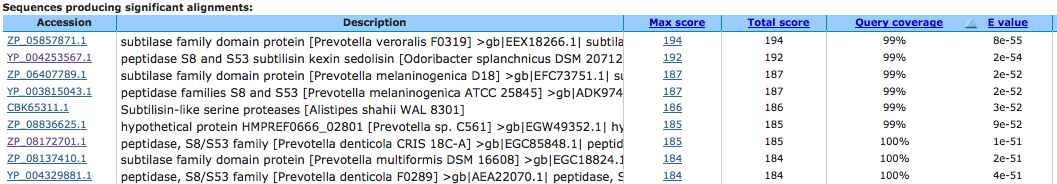
\includegraphics[width=0.8\textwidth]{blastp.png}
\end{center}
\vspace{0.5cm}

\item What is the possible function of the protein encoded by \texttt{fragment\_007}?

\texttt{fragment\_007} encodes for a subtilase family domain protein. It is a member of the peptidases S8 (subtilisin and kexin) and S53 (sedolisin) family. These include endopeptidases and exopeptidases.

\item Which species is most predominant in your BLAST output?

\emph{Prevotella} species

\item Could you have obtained the same results using another BLAST program, without having to translate the nucleotide sequence of \texttt{fragment\_007}?

Yes, using blastx

\item How do results from Protein BLAST compare with the results from Nucleotide BLAST?

Amino acid sequences are more conserved than nucleotide sequences. Often even the highest-scoring subject sequences retrieved using the nucleotide sequence will cover only small regions of the query sequence, while quite often the corresponding sequences retrieved using the amino acid sequence will cover more of the gene.

\end{enumerate}

\section{Finding orthologs}

Putative ortholog of \emph{Saccharomyces cerevisiae} Pho2p in \emph{Candida glabrata}?

\texttt{CAGL0L07436g}

Are the findings of the paper consistent with your observations?

Yes

\end{document}
